% Centinela Orinoco — artículo en formato IEEE (IEEEtran, conferencia)
% Compilar en Overleaf con pdfLaTeX (subir el zip con main.tex y las figuras fig-*).
\documentclass[conference]{IEEEtran}

\usepackage[T1]{fontenc}
\usepackage[utf8]{inputenc}
\usepackage[spanish,es-tabla,es-nodecimaldot,es-noshorthands]{babel}
\usepackage{amsmath,amssymb}
\usepackage{graphicx}
\usepackage{booktabs}
\usepackage{array}
\usepackage{xcolor}
\usepackage{tikz}
\usetikzlibrary{positioning,arrows.meta,fit,backgrounds}
\usepackage{url}
\usepackage[hidelinks]{hyperref}

\newcommand{\pend}[1]{\textcolor{red}{[#1]}}
\newcommand{\sicheck}{\ensuremath{\checkmark}}
\newcommand{\nocheck}{--}

\begin{document}

\title{Centinela Orinoco: arquitectura de datos inteligente para la detección temprana de la minería ilegal en el Arco Minero del Orinoco\\
\large Centinela Orinoco: An Intelligent Data Architecture for Early Detection of Illegal Mining in Venezuela's Orinoco Mining Arc}

\author{
\IEEEauthorblockN{Julio Cesar Canelón Rangel, José Francisco Escalante Rosales y Miguel Damián Mota Garrido}
\IEEEauthorblockA{Maestría en Tecnologías de la Información\\
Universidad Nacional Experimental de Guayana (UNEG), Puerto Ordaz, Venezuela\\
juliocanelon@gmail.com, jescalante.ve@gmail.com, mmotal@gmail.com}
}

\maketitle

\begin{abstract}
La minería aurífera no regulada en el sur de Venezuela causa deforestación, sedimentación de ríos y contaminación por mercurio que afecta a pueblos indígenas y al embalse de Guri. La causa de fondo es una asimetría de información: los datos satelitales, de campo, comunitarios y científicos existen, pero se consultan por separado y con días de retraso. Este artículo presenta Centinela Orinoco, una arquitectura de datos inteligente de cuatro capas inscrita en la iniciativa AmazonIA~4.0. La capa de ingesta automatiza la captura de anomalías térmicas (NASA FIRMS), catálogos Sentinel-1, -2 y -3 (Copernicus), niveles hidrológicos (INAMEH), formularios de patrullaje y denuncias anónimas, sin duplicados y con reanudación tras fallos. La capa de almacenamiento combina PostgreSQL con PostGIS y pgvector, MongoDB y un almacén de objetos, coordinados por una saga compensable con idempotencia. La capa de inteligencia implementa una memoria semántica georreferenciada (RAG espacial) que combina embeddings de Gemini en pgvector con un filtro espacial de PostGIS y un reranker de puntaje compuesto, más una cascada de modelos de lenguaje con respaldo determinístico. La capa de consumo ofrece un tablero web con mapa táctico, incidentes y boletines. El diseño incluye nodos de borde con almacenamiento local y MQTT/LoRaWAN para operar con cortes de red y energía. El prototipo implementa la ingesta real, la persistencia políglota, la búsqueda vectorial espacial y el canal comunitario; el análisis de píxeles y la orquestación con Airflow quedan como trabajo inmediato.
\end{abstract}

\begin{IEEEkeywords}
arquitectura de datos inteligente, generación aumentada por recuperación, minería ilegal, teledetección, computación en el borde, Arco Minero del Orinoco, AmazonIA~4.0.
\end{IEEEkeywords}

% ---------------------------------------------------------------------------
\section{Introducción}

La cuenca amazónica regula el clima de Sudamérica y alberga más de una cuarta parte de la biodiversidad terrestre. La minería aurífera es uno de sus principales motores de degradación: en la Amazonía brasileña la deforestación inducida por la minería se extiende hasta 70~km más allá de las concesiones~\cite{sonter2017}, y el auge reciente de la minería ilegal acelera la pérdida de bosque en tierras indígenas y áreas protegidas~\cite{siqueira2021}. En Madre de Dios (Perú) se ha documentado la pérdida acelerada de bosques protegidos durante más de tres décadas~\cite{asner2017,caballero2018}.

Los efectos no se limitan al bosque. El mercurio usado en la amalgamación se acumula en el dosel de los bosques cercanos a la minería artesanal~\cite{gerson2022} y en el aire de las zonas mineras venezolanas~\cite{garcia2006}, y los sedimentos removidos elevan la turbidez de los ríos~\cite{lobo2015}. En Venezuela, la Zona de Desarrollo Estratégico Nacional Arco Minero del Orinoco (AMO), creada en 2016 sobre 111\,843,70~km² al sur del Orinoco, cerca del 12,2\,\% del territorio nacional~\cite{decreto2248}, se superpone con las cuencas del Caroní, el Caura y el Cuyuní, y con territorios de los pueblos pemón, ye'kwana, sanemá y piaroa. Su implementación aumentó la vulnerabilidad del territorio~\cite{colmenares2024} y los conflictos en áreas protegidas como el Parque Nacional Canaima~\cite{rodriguez2023}. En el estado Amazonas la minería opera incluso dentro del Parque Nacional Yapacana.

Hoy la detección depende de patrullajes, de denuncias por canales informales y de revisiones satelitales puntuales. Cada fuente se consulta por separado, sin correlación espacial, y la decisión de intervenir se toma de forma manual. El problema central no es la falta de datos, sino la \emph{asimetría de información}: no existe una infraestructura que integre en tiempo casi real esas fuentes heterogéneas. Las revisiones sobre IA para ecosistemas regionales~\cite{pimenow2025} y sobre tecnologías inteligentes para la resiliencia climática~\cite{debruyn2026} coinciden en que la tecnología solo aporta si se integra con la gobernanza del territorio.

Este trabajo responde a la pregunta: \emph{¿qué arquitectura de datos permite integrar fuentes satelitales, de campo, comunitarias y científicas para detectar a tiempo la minería ilegal en el sur de Venezuela, con conectividad intermitente y protegiendo los datos de las comunidades indígenas?} Se inscribe en la iniciativa AmazonIA~4.0, que propone el desarrollo sostenible de la Amazonía mediante tecnologías de la Cuarta Revolución Industrial, y en la Estrategia del Programa sobre el Hombre y la Biosfera (MAB) de la UNESCO y su Plan de Acción de Lima~\cite{unesco2017}, que orientan la gestión de las reservas de biosfera, entre ellas la de Alto Orinoco-Casiquiare, en el estado Amazonas.

Las contribuciones son:
\begin{enumerate}
\item Una arquitectura por capas con persistencia políglota y una saga compensable que mantiene la consistencia entre motores.
\item Una memoria semántica georreferenciada que combina similitud vectorial y filtro espacial en una sola consulta, con un reranker de puntaje compuesto.
\item Un filtro semántico territorial (\emph{geofencing}) que rechaza documentos ajenos a la Amazonía venezolana antes de incorporarlos al corpus.
\item Una estrategia \emph{offline-first} para puestos remotos y una política de anonimización alineada con los principios CARE.
\item Un prototipo funcional con ingesta real de cinco fuentes satelitales e hidrológicas.
\end{enumerate}

El resto del artículo se organiza así: la Sección~\ref{sec:rel} revisa los trabajos relacionados; la Sección~\ref{sec:arq} describe la arquitectura; la Sección~\ref{sec:impl}, el prototipo; la Sección~\ref{sec:res} discute los resultados y limitaciones, y la Sección~\ref{sec:conc} concluye.

% ---------------------------------------------------------------------------
\section{Trabajos relacionados}\label{sec:rel}

\subsection{Teledetección de la minería}
Camalan \emph{et al.}~\cite{camalan2022} detectan cambios por minería aluvial con redes profundas sobre Sentinel-2, pero el sensor óptico depende de la nubosidad, muy alta en la Guayana. Pereira \emph{et al.}~\cite{pereira2024} usan el radar Sentinel-1 y algoritmos de detección de embarcaciones para identificar dragas flotantes, lo que funciona con cualquier cobertura de nubes. Caballero Espejo \emph{et al.}~\cite{caballero2018} y Lobo \emph{et al.}~\cite{lobo2015} construyen series Landsat de largo plazo. Valbuena Gaona \emph{et al.}~\cite{valbuena2024} proponen una herramienta de alertas de deforestación y minería basada en teledetección. Todos trabajan con una sola familia de datos y no corroboran con información de campo.

\subsection{IA, Big Data y soporte a la decisión}
Vishwakarma \emph{et al.}~\cite{vishwakarma2025} muestran que la analítica en tiempo casi real previene brechas normativas en cadenas de suministro. Arafat \emph{et al.}~\cite{arafat2025} sistematizan las cinco V del Big Data, que aquí se usan para caracterizar las fuentes. Le y Fan~\cite{le2024} revisan los gemelos digitales y la sincronización de datos IoT con un modelo en la nube.

\subsection{Recuperación semántica y borde}
La generación aumentada por recuperación (RAG) condiciona un modelo de lenguaje con documentos recuperados~\cite{lewis2020,gao2023}; los índices HNSW permiten buscar vecinos aproximados en grandes colecciones~\cite{malkov2020}. MQTT y LoRaWAN se han combinado para el monitoreo ambiental en tiempo real con bajo consumo~\cite{rosli2020}. Los principios CARE orientan la gobernanza de datos indígenas~\cite{carroll2020}.

\subsection{Brechas}
La Tabla~\ref{tab:comp} resume la comparación. Ningún antecedente correlaciona satélite, campo, comunidad y literatura científica; ninguno incorpora memoria semántica georreferenciada ni opera con conectividad intermitente, y la gobernanza indígena aparece solo de forma tangencial. La literatura indexada específica de la Amazonía venezolana es además escasa, lo que refuerza la pertinencia del caso.

\begin{table}[!t]
\caption{Comparación de antecedentes. En este trabajo, la operación offline está en diseño}
\label{tab:comp}
\centering
\footnotesize
\setlength{\tabcolsep}{3pt}
\begin{tabular}{@{}l l c c c c c@{}}
\toprule
Ref. & Datos & Multi- & RAG & T. casi & Offline & Gob. \\
 & & fuente & & real & & indígena \\
\midrule
\cite{camalan2022} & Sentinel-2 & \nocheck & \nocheck & \nocheck & \nocheck & \nocheck \\
\cite{pereira2024} & Sentinel-1 & \nocheck & \nocheck & \nocheck & \nocheck & \nocheck \\
\cite{caballero2018} & Landsat & \nocheck & \nocheck & \nocheck & \nocheck & \nocheck \\
\cite{valbuena2024} & Teledetección & \nocheck & \nocheck & parcial & \nocheck & \nocheck \\
\cite{siqueira2021} & Deforestación & \nocheck & \nocheck & \nocheck & \nocheck & parcial \\
\cite{vishwakarma2025} & Operacionales & \sicheck & \nocheck & \sicheck & \nocheck & \nocheck \\
\cite{le2024} & IoT & \sicheck & \nocheck & \sicheck & \nocheck & \nocheck \\
\midrule
\textbf{Este trabajo} & \textbf{Sat.+campo+} & \sicheck & \sicheck & \sicheck & \sicheck & \sicheck \\
 & \textbf{com.+corpus} & & & & & \\
\bottomrule
\end{tabular}
\end{table}

% ---------------------------------------------------------------------------
\section{Arquitectura propuesta}\label{sec:arq}

La Fig.~\ref{fig:arq} muestra las capas, desde la captura en campo hasta el consumo, con la gobernanza como capa transversal. A lo largo del texto se distingue lo \textbf{implementado} en el prototipo de lo que está \textbf{en diseño}.

\begin{figure*}[!t]
\centering
\begin{tikzpicture}[
  font=\footnotesize,
  box/.style={draw, rounded corners=2pt, align=center, minimum height=7mm, text width=25mm, fill=white},
  dbox/.style={box, dashed},
  layer/.style={draw, rounded corners=4pt, fill=gray!8, inner sep=4pt},
  arr/.style={-{Stealth[length=2mm]}, thick},
  lab/.style={font=\footnotesize\bfseries, anchor=south}
]
% Fuentes
\node[box] (f1) {NASA FIRMS};
\node[box, below=2mm of f1] (f2) {Sentinel-1/2/3};
\node[box, below=2mm of f2] (f3) {INAMEH (PDF)};
\node[box, below=2mm of f3] (f4) {Kobo / ODK};
\node[box, below=2mm of f4] (f5) {Denuncias\\comunitarias};
\node[box, below=2mm of f5] (f6) {Corpus científico};
\node[dbox, below=2mm of f6] (f7) {Sensores LoRaWAN};
% Ingesta
\node[box, right=7mm of f2] (i1) {Scheduler\\satelital};
\node[box, below=2mm of i1] (i2) {API REST\\y webhooks};
\node[dbox, below=2mm of i2] (i3) {Nodo de borde\\SQLite + MQTT};
\node[dbox, below=2mm of i3] (i4) {Apache Kafka};
% Almacenamiento
\node[box, right=7mm of i1] (s1) {PostgreSQL\\PostGIS + pgvector};
\node[box, below=2mm of s1] (s2) {MongoDB\\(evidencias)};
\node[box, below=2mm of s2] (s3) {Almacén de objetos};
\node[dbox, below=2mm of s3] (s4) {Lakehouse Delta/MinIO\\+ Spark};
% Inteligencia
\node[box, right=7mm of s1] (a1) {Cascada LLM\\+ contingencia};
\node[box, below=2mm of a1] (a2) {RAG espacial\\+ reranker};
\node[box, below=2mm of a2] (a3) {Geofencing\\semántico};
\node[dbox, below=2mm of a3] (a4) {Motor de reglas\\Airflow};
% Consumo
\node[box, right=7mm of a1] (c1) {Mapa táctico};
\node[box, below=2mm of c1] (c2) {Incidentes};
\node[box, below=2mm of c2] (c3) {Boletines IA};
\node[box, below=2mm of c3] (c4) {Chat operativo};

\begin{scope}[on background layer]
\node[layer, fit=(f1)(f7)] (L1) {};
\node[layer, fit=(i1)(i4)] (L2) {};
\node[layer, fit=(s1)(s4)] (L3) {};
\node[layer, fit=(a1)(a4)] (L4) {};
\node[layer, fit=(c1)(c4)] (L5) {};
\end{scope}
\node[lab] at (L1.north) {Fuentes};
\node[lab] at (L2.north) {1. Ingesta};
\node[lab] at (L3.north) {2. Almacenamiento};
\node[lab] at (L4.north) {3. Inteligencia};
\node[lab] at (L5.north) {4. Consumo};

\draw[arr] (L1.east |- i2) -- (L2.west |- i2);
\draw[arr] (L2.east |- s2) -- (L3.west |- s2);
\draw[arr] (L3.east |- a2) -- (L4.west |- a2);
\draw[arr] (L4.east |- c2) -- (L5.west |- c2);

\node[draw, rounded corners=4pt, fill=gray!20, below=4mm of L1.south west, anchor=north west,
      minimum width=0pt, text width=165mm, align=center, inner sep=3pt] (gov)
  {Gobernanza transversal: RLS y RBAC · denuncia anónima por defecto · geo-enmascaramiento · principios CARE · trazabilidad por hash (blockchain, diseño)};
\end{tikzpicture}
\caption{Arquitectura de Centinela Orinoco. Los bloques de borde continuo están implementados en el prototipo; los de borde discontinuo están en diseño.}
\label{fig:arq}
\end{figure*}

\subsection{Capa de ingesta}
La Tabla~\ref{tab:fuentes} caracteriza las fuentes según la dimensión del Big Data que domina en cada una~\cite{arafat2025}. Un \emph{scheduler} en proceso ejecuta una tarea por fuente con cadencia de producción. Para Sentinel se ingiere el catálogo de escenas (huella, órbita, nubosidad, polarización), no los píxeles. Cada ejecución inserta solo registros nuevos mediante claves de conflicto por fuente (por ejemplo, satélite, latitud, longitud, fecha y hora para FIRMS), descarta los registros cuyo centro cae fuera de Amazonas, Bolívar, Delta Amacuro o la Guayana Esequiba, y queda registrada en una tabla de ejecuciones con los conteos de recibidos, insertados y omitidos. La próxima ejecución se calcula desde esa tabla, de modo que la cadencia sobrevive a reinicios.

Las minutas de patrullaje llegan por \emph{webhooks} de KoboToolbox y ODK; las denuncias, por una API que valida coordenadas y sube la evidencia a un depósito privado. El corpus científico se ingiere desde PDF o DOI: se extrae el texto, se consultan los metadatos en Crossref y un modelo de lenguaje decide si el documento es pertinente para la Amazonía venezolana; si no lo es, se rechaza con HTTP~400.

En el diseño objetivo, el scheduler se sustituye por productores que publican en tópicos de Apache Kafka (\texttt{firms.raw}, \texttt{s1.raw}, \texttt{telemetry.raw}, \texttt{field.reports}), lo que permite reprocesar desde el registro y escalar por partición.

\begin{table}[!t]
\caption{Fuentes de datos ingeridas}
\label{tab:fuentes}
\centering
\footnotesize
\setlength{\tabcolsep}{3pt}
\begin{tabular}{@{}p{24mm} p{24mm} l l@{}}
\toprule
Fuente & Dato & Cadencia & V dominante \\
\midrule
NASA FIRMS (VIIRS, MODIS) & Anomalías térmicas & 3~h & Velocidad \\
Sentinel-1 GRD & Catálogo SAR & 12~h & Volumen \\
Sentinel-2 L2A & Catálogo óptico & 24~h & Volumen \\
Sentinel-3 OLCI/SLSTR & Productos de agua & 24~h & Volumen \\
INAMEH & Cota del Orinoco (4 estaciones) & 6~h & Veracidad \\
Kobo / ODK & Formularios, fotos, GPS & Evento & Variedad \\
Denuncias & Texto, imagen, video & Evento & Variedad \\
Corpus científico & PDF, DOI & Evento & Valor \\
\bottomrule
\end{tabular}
\end{table}

\subsection{Almacenamiento políglota y consistencia}
Cada dato se guarda en el motor que mejor se ajusta a su forma. PostgreSQL guarda denuncias, incidentes y operaciones, con restricciones de integridad; PostGIS indexa las geometrías; pgvector guarda los vectores de los documentos RAG junto a su geometría. MongoDB guarda la evidencia heterogénea con esquema versionado, y los binarios van a un almacén de objetos, con su ruta y su hash SHA-256 registrados en MongoDB.

Elevar una denuncia a incidente escribe en PostgreSQL y en MongoDB. Para evitar estados parciales se usa el patrón \emph{saga}: una función almacenada crea el incidente bajo bloqueo de fila, la API escribe la evidencia en MongoDB con \emph{upsert} y, si esta escritura falla tras un número configurable de reintentos, una acción compensatoria cancela el incidente, devuelve la denuncia a su estado anterior y la API responde HTTP~503. Cada operación lleva una \texttt{Idempotency-Key}; repetirla con el mismo cuerpo devuelve la respuesta guardada, y repetirla con otro cuerpo devuelve HTTP~409. Ante la caída de MongoDB, el sistema prefiere no confirmar antes que quedar inconsistente.

En el diseño objetivo, un Lakehouse Delta Lake sobre MinIO guarda el histórico en zonas Bronze (crudo), Silver (validado y deduplicado) y Gold (agregados por sector y día), procesadas con PySpark.

\subsection{Memoria semántica georreferenciada}
Se vectorizan cuatro tipos de conocimiento: fragmentos del corpus científico con sus coordenadas y mediciones (Hg, turbidez, hectáreas deforestadas), narrativas generadas por el scheduler para los focos relevantes y las lecturas hidrológicas, minutas de campo y normativa del AMO y de las áreas protegidas.

Cada documento se vectoriza con el modelo \texttt{gemini-embedding-001} de Google, reducido a 768 dimensiones y normalizado; los documentos usan el tipo de tarea \emph{retrieval document} y las consultas, \emph{retrieval query}. Los documentos se insertan sin vector y un proceso del servidor los vectoriza por lotes al arrancar, después de cada ingesta y al ingresar un documento al corpus. Así, un fallo o una cuota agotada en Gemini nunca bloquea la ingesta: lo pendiente se completa en la siguiente pasada.

Se elige pgvector con índice HNSW~\cite{malkov2020} en lugar de una base vectorial dedicada porque permite filtrar por similitud coseno y por distancia geodésica (\texttt{ST\_DWithin}) en una sola consulta SQL, sin sincronizar dos almacenes ni enviar coordenadas de comunidades a un servicio externo. La consulta recupera los $k$ vecinos más cercanos dentro de un radio $R$, descarta los de similitud menor que 0,65 y los reordena con el puntaje compuesto
\begin{equation}
\label{eq:score}
S = 0{,}45\,s + 0{,}20\left(1-\frac{d}{R}\right) + 0{,}15\,e^{-t/90} + 0{,}10\,a + 0{,}10\,v,
\end{equation}
donde $s$ es la similitud coseno, $d$ la distancia en km, $t$ la antigüedad en días, $a\in\{0,1\}$ indica si la fuente es arbitrada y $v\in[0,1]$ es la severidad. La similitud domina porque es la señal principal de pertinencia; la proximidad y la recencia (vida media de unos 62~días) priorizan la evidencia cercana y la actividad minera activa. Los pesos son iniciales y deben calibrarse con un conjunto etiquetado. Los documentos que superan el filtro alimentan a un modelo de lenguaje que sintetiza la respuesta con citas~\cite{lewis2020,gao2023}. Si no es posible vectorizar la consulta, la búsqueda vuelve a la coincidencia de términos con distancia geodésica.

La generación usa una cascada de cuatro modelos Gemini con cuotas diarias: ante un error de cuota o HTTP~429 el modelo se marca como agotado y se pasa al siguiente; si todos fallan, se devuelve una respuesta determinística de contingencia.

\subsection{Flujo dinámico automatizado}
La Tabla~\ref{tab:reglas} define las reglas de decisión que, en el diseño objetivo, ejecutaría un DAG de Apache Airflow después de ingerir y correlar espacialmente las fuentes. La regla central exige la coincidencia de dos sensores independientes, porque un foco térmico aislado no prueba minería: puede ser una quema agrícola. En ese diseño, cada tarea de ingesta tendría tres reintentos con espera exponencial, y el fallo de una fuente no bloquearía las demás ramas. En el prototipo, un \emph{scheduler} propio ejecuta la ingesta de forma independiente por fuente y, si una falla, registra el error y la reintenta en su siguiente ejecución programada; las reglas aún no se aplican, porque R1 a R3 requieren el análisis de píxeles satelitales.

\begin{table}[!t]
\caption{Reglas de decisión del diseño objetivo (umbrales iniciales)}
\label{tab:reglas}
\centering
\footnotesize
\setlength{\tabcolsep}{3pt}
\begin{tabular}{@{}l p{45mm} p{22mm}@{}}
\toprule
\# & Condición & Acción \\
\midrule
R1 & Foco FIRMS de confianza alta y caída de retrodispersión S1 $\geq$ 3~dB a $\leq$ 2~km, en área protegida o a $\leq$ 5~km de territorio indígena & Incidente crítico, boletín y notificación \\
R2 & Turbidez $>$ 100~NTU sostenida 3~h aguas arriba de Guri & Incidente alto por sedimentación \\
R3 & Caída de NDVI $\geq$ 30\,\% respecto a la mediana de 90 días & Incidente medio; verificar con S1 \\
R4 & Denuncia con $\geq$ 2 evidencias a $\leq$ 3~km de un foco de los últimos 7 días & Priorizar validación \\
R5 & Foco FIRMS aislado & Solo bitácora \\
\bottomrule
\end{tabular}
\end{table}

\subsection{Resiliencia de red (offline-first)}
En los puestos de Guardería, un nodo de borde (Raspberry Pi o Jetson, con panel solar y batería) recibe los sensores por LoRaWAN y las tabletas Kobo/ODK por WiFi local, guarda en SQLite y MinIO local, y reenvía por MQTT con QoS~1 y sesión persistente cuando hay enlace satelital~\cite{rosli2020}. La cola prioriza las alertas críticas, luego la telemetría agregada y por último los binarios comprimidos. Del lado del servidor, la idempotencia permite reintentar sin duplicar, y como FIRMS publica ventanas de dos días y STAC de cuatro, la siguiente ejecución recupera lo que faltó tras una caída.

\subsection{Gobernanza y privacidad}
La denuncia es anónima por defecto, y una restricción de la base de datos impide guardar nombre o contacto cuando lo es. Los datos de contacto nunca salen de PostgreSQL, los registros no contienen datos personales y la seguridad a nivel de fila (RLS) restringe el acceso al \emph{backend}. El diseño agrega control de acceso por roles (administrador, operador, analista, comunidad), generalización de coordenadas de comunidades a 0,01° (unos 1,1~km), eliminación de metadatos EXIF y consentimiento comunitario previo según los principios CARE~\cite{carroll2020}. El hash SHA-256 de cada evidencia puede registrarse en una cadena de bloques permisionada para demostrar ante las autoridades que no fue alterada.

\subsection{Despliegue objetivo en la nube}
El prototipo corre hoy en servicios gestionados (Cloud Run, Supabase y MongoDB Atlas) sin contenedores propios. Para producción institucional se propone una arquitectura en AWS que conserva los mismos flujos funcionales (Tabla~\ref{tab:aws}). La API se empaqueta en contenedores sobre Amazon ECS con Fargate y escala de forma horizontal; los conectores de ingesta pasan a funciones AWS Lambda disparadas por Amazon EventBridge Scheduler, y AWS Step Functions orquesta las dependencias y los reintentos que hoy se resuelven reprogramando la tarea en el \emph{scheduler}. Las credenciales de las fuentes se guardan en AWS Secrets Manager, los objetos y volúmenes se cifran con AWS KMS, y Amazon CloudWatch y AWS CloudTrail registran métricas, alarmas y auditoría. En los puestos de Guardería, AWS IoT Greengrass ejecuta el nodo de borde con almacenamiento local y publica por MQTT hacia AWS IoT Core cuando hay enlace.

La memoria semántica se mantiene en PostgreSQL: Amazon Aurora PostgreSQL admite PostGIS y pgvector, de modo que la búsqueda vectorial y el filtro espacial siguen resolviéndose en una sola consulta. Una base vectorial aparte, como Amazon OpenSearch, solo se justificaría si el volumen de documentos superara lo que el índice HNSW de PostgreSQL maneja con la latencia requerida.

\begin{table*}[!t]
\caption{Correspondencia entre el prototipo y la arquitectura objetivo en AWS}
\label{tab:aws}
\centering
\footnotesize
\setlength{\tabcolsep}{4pt}
\begin{tabular}{@{}p{42mm} p{48mm} p{78mm}@{}}
\toprule
Componente actual & Servicio AWS objetivo & Función \\
\midrule
SPA React + Vite & Amazon CloudFront + S3 & Distribución de la interfaz web con TLS \\
Sin autenticación de usuarios & Amazon Cognito + AWS WAF & Identidad, RBAC por rol y filtrado de tráfico en el borde \\
API Express (Node.js) & Amazon API Gateway + ECS Fargate & API REST en contenedores con escalado horizontal \\
Scheduler en proceso & EventBridge Scheduler + AWS Lambda & Ejecución periódica de los conectores FIRMS, STAC/OData, INAMEH y corpus \\
Reprogramación tras fallos en el scheduler & AWS Step Functions & Orquestación con dependencias, reintentos y control de ejecución \\
Supabase PostgreSQL + PostGIS + pgvector & Amazon Aurora PostgreSQL & Datos relacionales, espaciales y vectoriales en un mismo motor \\
Supabase Storage & Amazon S3 & Evidencias privadas y zonas Bronze, Silver y Gold del Lakehouse \\
(no implementado) & AWS Glue Data Catalog + Amazon Athena & Catálogo y consulta analítica del Lakehouse \\
MongoDB Atlas & Amazon DocumentDB & Documentos de evidencia y auditoría de incidentes \\
Google Gemini (LLM y embeddings) & Gemini o Amazon Bedrock & Síntesis y embeddings; un cambio de modelo exige revectorizar \\
Nodo de borde (diseño) & AWS IoT Greengrass + IoT Core & Procesamiento local sin conexión y mensajería MQTT \\
Variables de entorno & Secrets Manager, KMS, IAM & Credenciales, cifrado y privilegio mínimo \\
Registros del servidor & CloudWatch + CloudTrail & Métricas, alarmas, trazas y auditoría \\
\bottomrule
\end{tabular}
\end{table*}

% ---------------------------------------------------------------------------
\section{Implementación del prototipo}\label{sec:impl}

El prototipo es una aplicación web con API en Node.js y Express (TypeScript) y una SPA en React~19 con Leaflet. Usa Supabase (PostgreSQL con PostGIS y pgvector), MongoDB Atlas y Supabase Storage, y está desplegado en Google Cloud Run mediante Google AI Studio (\url{https://centinela-orinoco-2026.ai.studio}). El código está en \url{https://github.com/juliocanelon/centinela-orinoco-2026}. La Tabla~\ref{tab:estado} resume el estado de cada componente. Las Figs.~\ref{fig:ui} a~\ref{fig:ia} muestran las vistas principales de la aplicación en producción: el mapa táctico (Fig.~\ref{fig:ui}), el panel de ingesta (Fig.~\ref{fig:ingesta}), los niveles del Orinoco (Fig.~\ref{fig:telemetria}), el canal de denuncias (Fig.~\ref{fig:veeduria}), el corpus científico georreferenciado (Fig.~\ref{fig:corpus}) y el análisis de zona (Fig.~\ref{fig:ia}).

\begin{table}[!t]
\caption{Estado de los componentes}
\label{tab:estado}
\centering
\footnotesize
\setlength{\tabcolsep}{3pt}
\begin{tabular}{@{}p{50mm} l@{}}
\toprule
Componente & Estado \\
\midrule
Ingesta real FIRMS, Sentinel-1/2/3 e INAMEH sin duplicados & Implementado \\
Persistencia políglota con saga e idempotencia & Implementado \\
Denuncias anónimas y elevación a incidente & Implementado \\
Corpus científico con geofencing semántico & Implementado \\
Cascada LLM con contingencia & Implementado \\
Densidad y priorización de focos & Implementado \\
Embeddings y búsqueda vectorial espacial & Implementado \\
Reranker de puntaje compuesto & Implementado \\
Análisis de píxeles (SAR, NDVI, turbidez) & Diseño \\
Kafka, Lakehouse, Spark, Airflow & Diseño \\
Nodo de borde, MQTT, LoRaWAN & Diseño \\
RBAC por rol y blockchain & Diseño \\
Pruebas unitarias (26 casos) & Implementado \\
Contenedores (Docker) & Pendiente \\
\bottomrule
\end{tabular}
\end{table}

\begin{figure*}[!t]
\centering
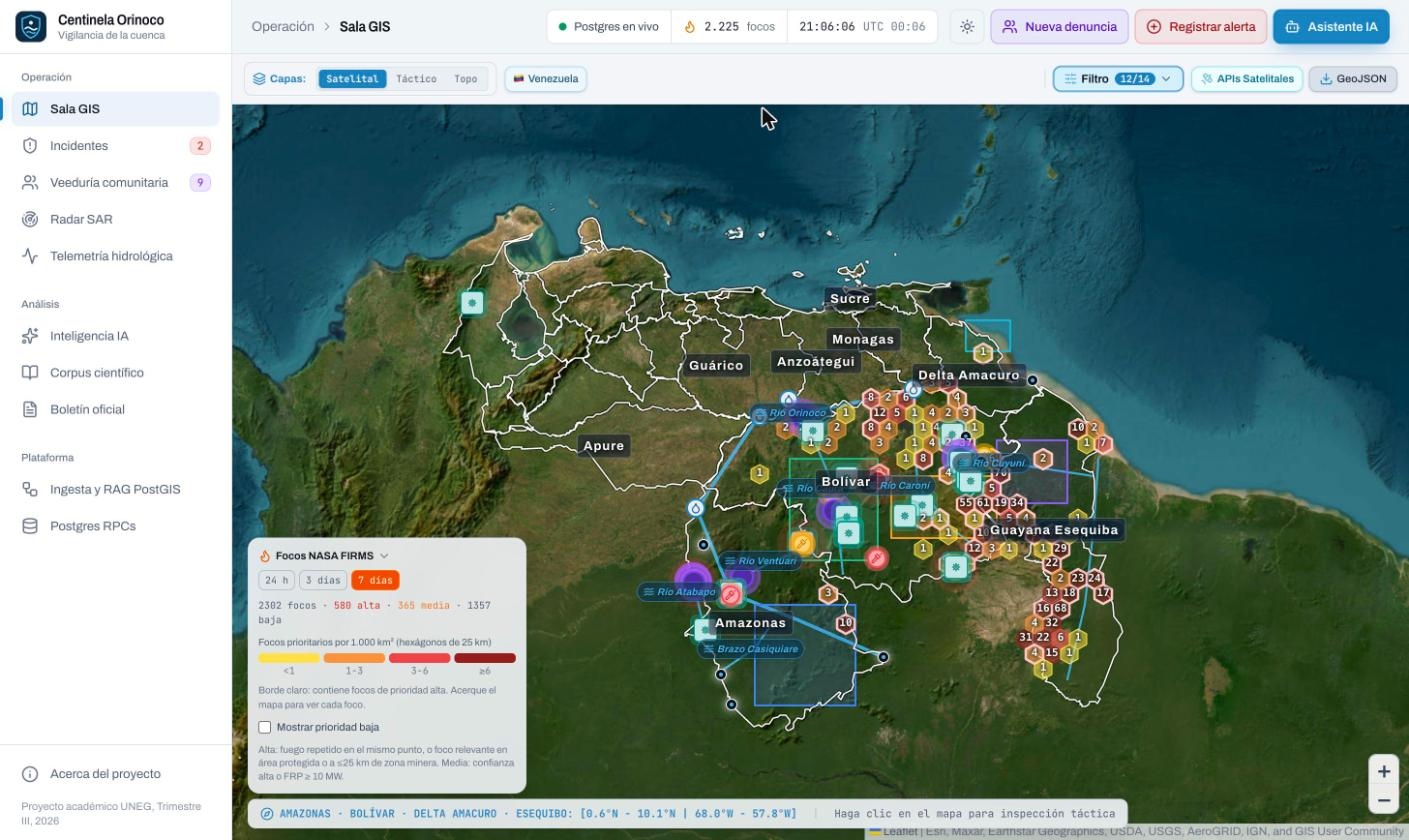
\includegraphics[width=\textwidth]{fig-sala-gis.jpg}
\caption{Sala GIS: mapa táctico con la densidad de focos NASA FIRMS de los últimos 7~días en hexágonos de 25~km, ríos, áreas protegidas y sectores mineros de referencia. Captura de la aplicación en producción, 25 de octubre de 2026.}
\label{fig:ui}
\end{figure*}

Para priorizar los focos térmicos sin que el tamaño de la celda distorsione la lectura, el mapa agrega los focos en una cuadrícula de hexágonos de 25~km de lado (unos 1\,624~km² cada uno) para ventanas de 1, 3 y 7~días. Un foco es relevante si su confianza es alta o su potencia radiativa es de al menos 10~MW. Un foco recibe prioridad alta si se repite en la misma celda de unos 1~km en al menos dos días distintos (actividad persistente, más propia de un frente minero que de una quema), o si es relevante y está dentro de una zona minera de referencia o a menos de 25~km de ella; los demás focos relevantes reciben prioridad media.

\begin{figure}[!t]
\centering
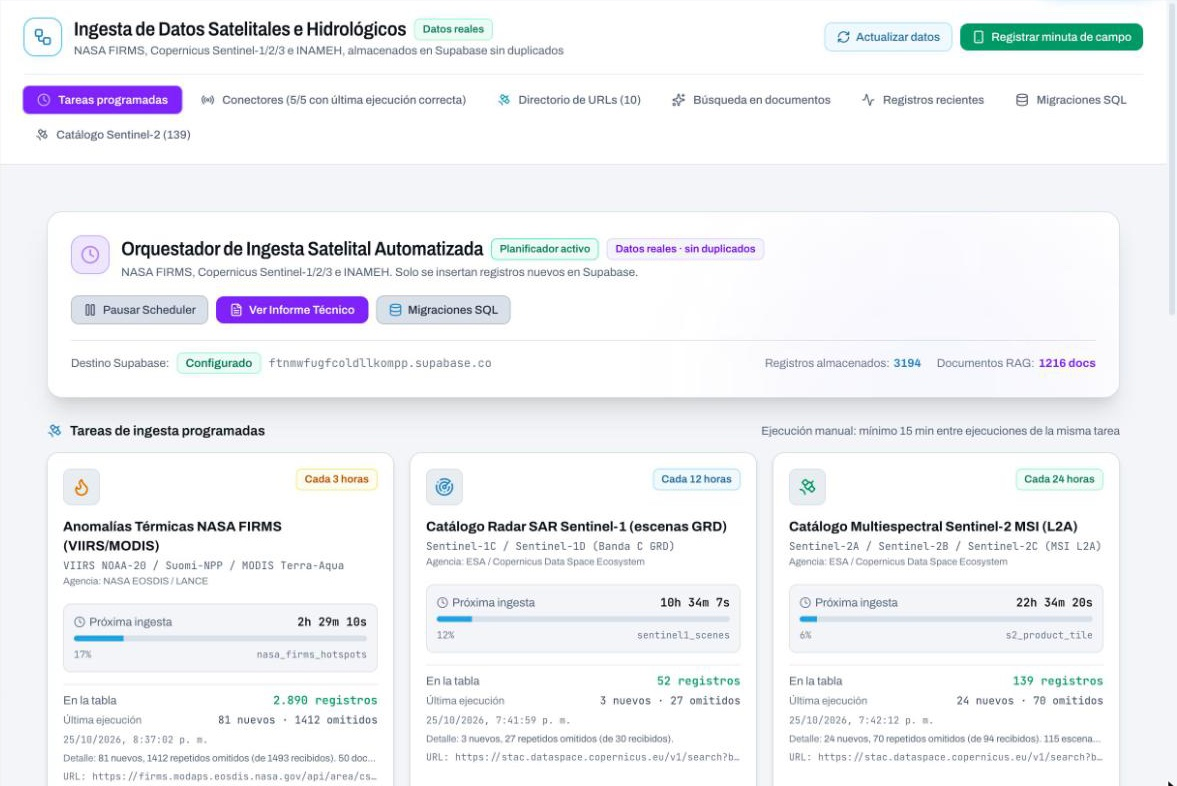
\includegraphics[width=\columnwidth]{fig-ingesta.jpg}
\caption{Panel de ingesta: tareas programadas por fuente con su cadencia, próxima ejecución y registros insertados y omitidos por duplicados.}
\label{fig:ingesta}
\end{figure}
\begin{figure}[!t]
\centering
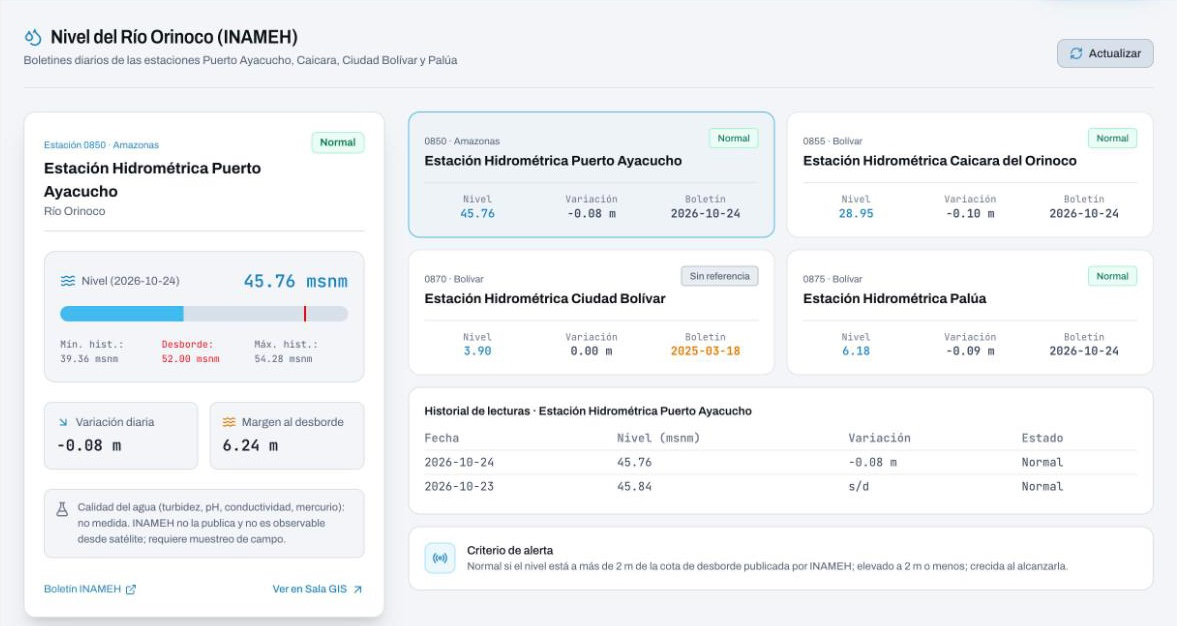
\includegraphics[width=\columnwidth]{fig-telemetria.jpg}
\caption{Niveles del río Orinoco extraídos de los boletines PDF del INAMEH para cuatro estaciones, con margen respecto a la cota de desborde.}
\label{fig:telemetria}
\end{figure}
\begin{figure}[!t]
\centering
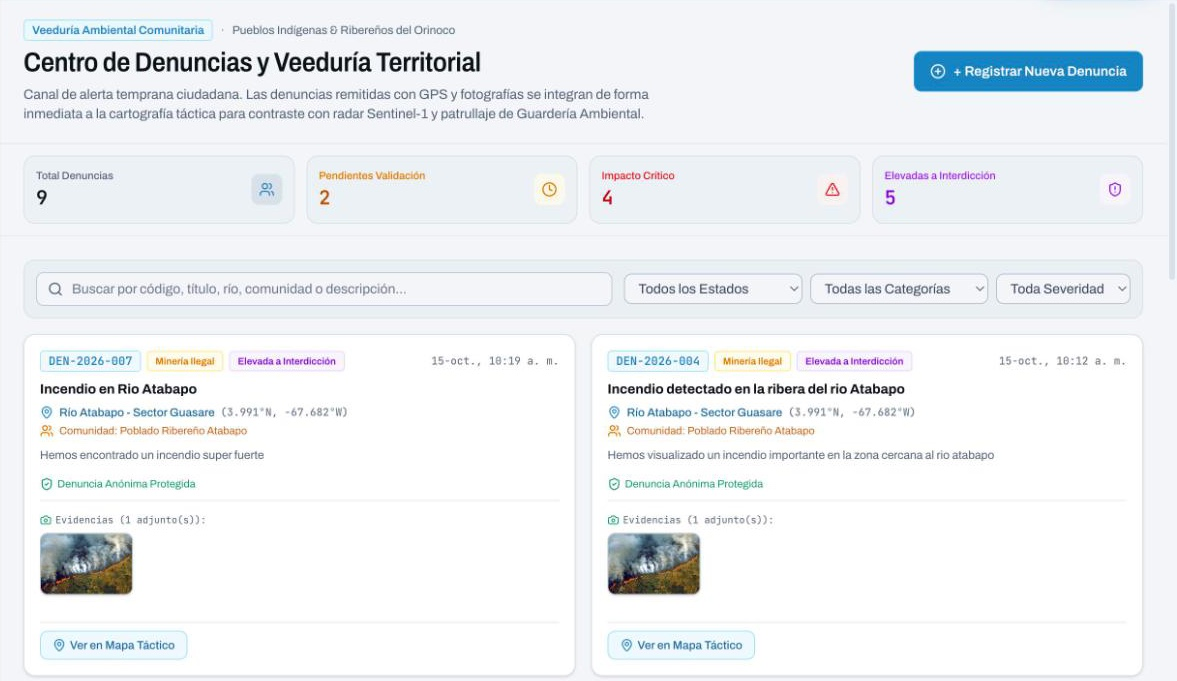
\includegraphics[width=\columnwidth]{fig-veeduria.jpg}
\caption{Canal de veeduría comunitaria: denuncias anónimas con geolocalización y evidencia fotográfica, elevables a incidente.}
\label{fig:veeduria}
\end{figure}
\begin{figure}[!t]
\centering
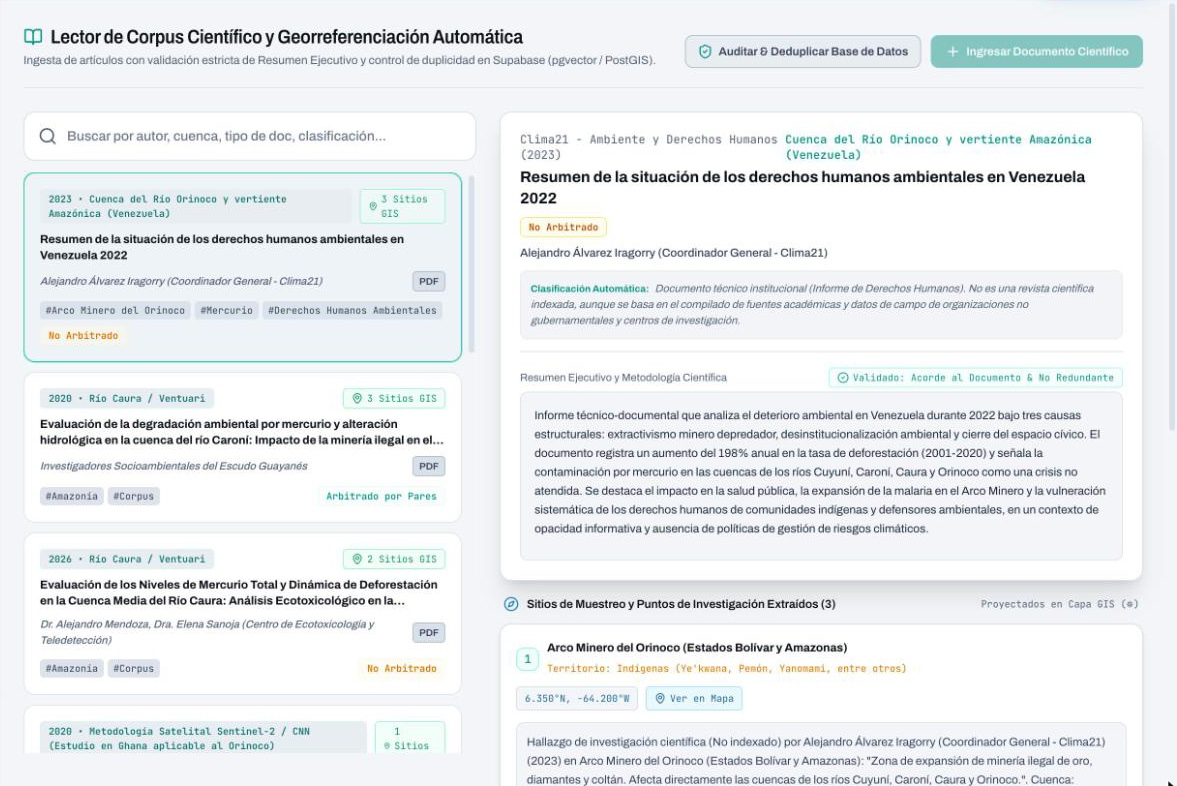
\includegraphics[width=\columnwidth]{fig-corpus.jpg}
\caption{Corpus científico: documentos clasificados automáticamente (arbitrado o no) con sus sitios de muestreo extraídos y proyectados en el mapa.}
\label{fig:corpus}
\end{figure}
\begin{figure}[!t]
\centering
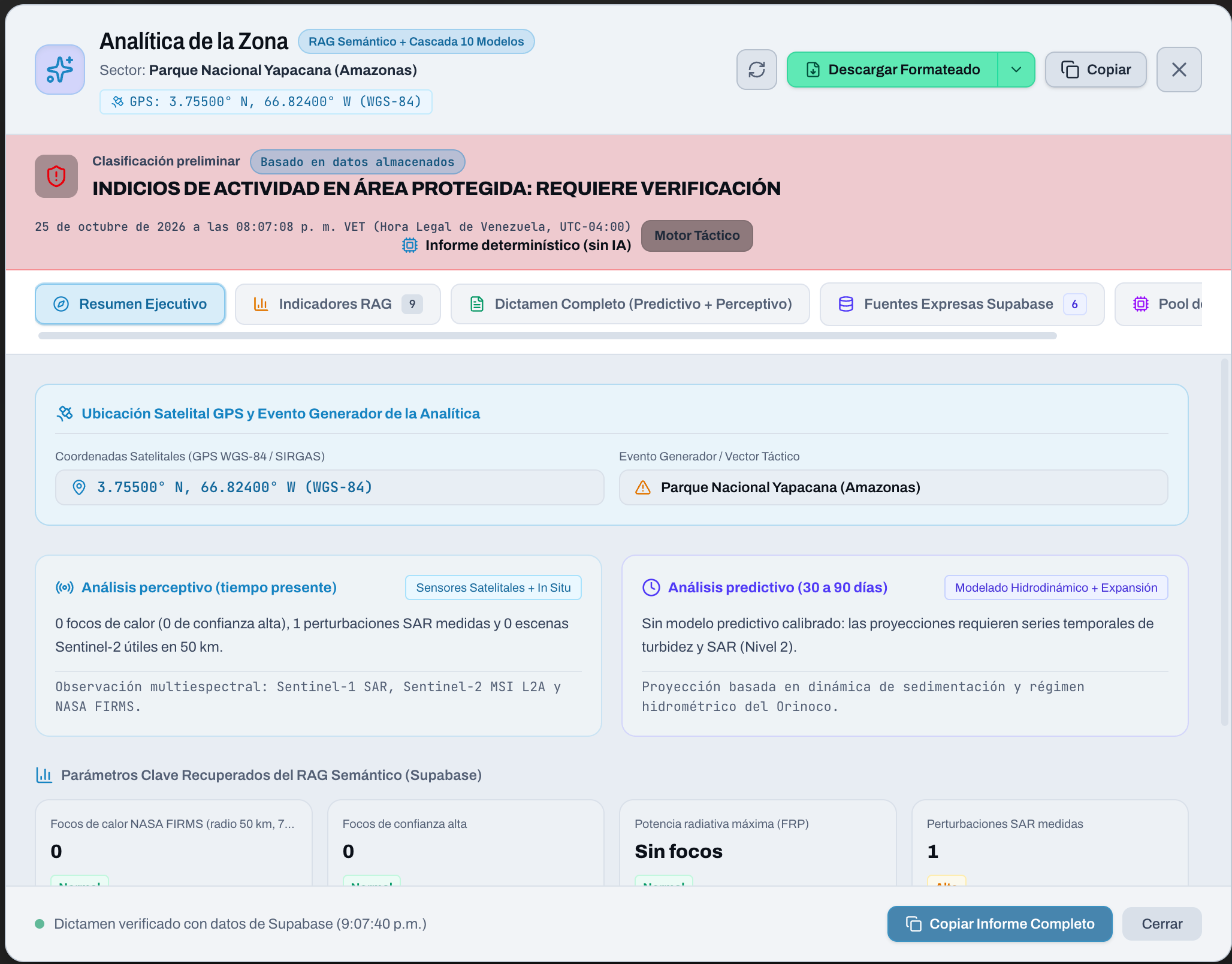
\includegraphics[width=\columnwidth]{fig-analitica-ia.png}
\caption{Análisis de zona para el Parque Nacional Yapacana. Al no responder la cascada de modelos, el sistema entregó el informe determinístico de contingencia («sin IA») calculado con los datos almacenados.}
\label{fig:ia}
\end{figure}

% ---------------------------------------------------------------------------
\section{Resultados y discusión}\label{sec:res}

\subsection{Verificación funcional}
La ingesta opera en producción con cadencia nominal y sin datos sintéticos desde el 24 de octubre de 2026. Al corte del 25 de octubre de 2026 (23:37~UTC), el sistema había almacenado 2\,890 focos FIRMS, 52 escenas Sentinel-1, 139 productos Sentinel-2, 105 productos Sentinel-3 y 8 lecturas hidrológicas del INAMEH, todos en los estados monitoreados, además de 1\,216 documentos en la memoria semántica. Las 25 ejecuciones más recientes terminaron con éxito. La deduplicación funciona en la práctica: en la última ejecución de FIRMS se recibieron 1\,493 focos, de los que 1\,412 ya estaban registrados y solo 81 se insertaron; en la misma consulta se descartaron 2\,538 focos fuera de los estados monitoreados, y 50 de los nuevos se clasificaron como relevantes (confianza alta o potencia radiativa $\geq$ 10~MW). En Sentinel-2 se descartaron 115 escenas cuyo centro cae fuera de la zona.

La saga está diseñada para tres casos: escritura exitosa, fallo de MongoDB (incidente cancelado y HTTP~503) y repetición de la clave de idempotencia con otro cuerpo (HTTP~409). El filtro territorial del corpus rechaza con HTTP~400 los documentos ajenos a la región. Las 26 pruebas unitarias actuales cubren la memoria semántica (embeddings, reranker, respaldo por texto y vectorización por lotes); la verificación automatizada de la saga y del filtro territorial queda pendiente.

\subsection{Memoria semántica}
La migración vectorial se aplicó en producción el 25 de octubre de 2026 y los 1\,216 documentos de la memoria semántica quedaron vectorizados. La vectorización respeta la cuota gratuita de Gemini, de 100 textos por minuto y 1\,000 por día: cuando se alcanza, el proceso se pausa y retoma solo al renovarse la cuota, mientras la ingesta sigue operando. Con esa cuota caben los cerca de 400 documentos diarios que genera FIRMS y las consultas de los usuarios.

En una prueba con documentos reales, la consulta ``contaminación por mercurio de la minería'' recuperó primero los artículos del corpus sobre mercurio en ríos con minería aurífera (similitud coseno de 0,72 a 0,74), y ``crecida del Orinoco'' recuperó las lecturas hidrológicas del INAMEH (0,69), aunque ninguno de esos documentos contiene la palabra ``crecida''. En cambio, la consulta ``incendios o actividad térmica cerca del río Atabapo'', con un radio de 100~km, no superó el umbral de 0,65 con ninguno de los cuatro documentos de esa zona y se resolvió con la búsqueda por texto, lo que indica que el umbral debe calibrarse con un conjunto de consultas etiquetadas.


\subsection{Aporte frente a los antecedentes}
A diferencia de los trabajos de un solo sensor~\cite{camalan2022,pereira2024,caballero2018}, el sistema registra en un mismo esquema espacial las anomalías térmicas, el catálogo de radar y óptico, los niveles del río, los reportes de campo y la literatura científica. Esa integración es la condición para aplicar reglas multisensor como R1, que reducen las falsas alarmas de un foco aislado. El canal anónimo responde a la falta de participación comunitaria señalada en~\cite{siqueira2021}, y la saga resuelve un problema que los antecedentes no tratan: la consistencia entre motores de almacenamiento distintos.

\subsection{Limitaciones}
El umbral de similitud y los pesos del reranker no están calibrados, y la cuota gratuita de embeddings limita a 1\,000 los documentos que se pueden vectorizar por día, lo que exigiría un plan de pago si el volumen creciera. Para Sentinel se registra el catálogo, pero no se analizan los píxeles, por lo que las reglas R1 a R3 no pueden evaluarse. Tampoco están calibrados los umbrales de la Tabla~\ref{tab:reglas}. INAMEH no publica turbidez ni mercurio, de modo que R2 depende de sensores propios. Faltan pruebas automatizadas de la saga y la validación en campo con la Guardería Ambiental.

% ---------------------------------------------------------------------------
\section{Conclusiones y trabajo futuro}\label{sec:conc}

Centinela Orinoco muestra que es posible atacar la asimetría de información sobre la minería ilegal en el sur de Venezuela con datos abiertos y software libre. El prototipo integra hoy cinco fuentes satelitales e hidrológicas reales, denuncias comunitarias anónimas y un corpus científico filtrado por pertinencia territorial en una memoria semántica vectorial y georreferenciada, con persistencia políglota consistente y degradación controlada ante fallos de red, de base de datos o de los modelos de lenguaje.

El trabajo inmediato es calibrar el umbral de similitud y los pesos del reranker con consultas etiquetadas; extender las pruebas a la saga y a los datos corruptos o vacíos; contenedorizar la API como primer paso hacia la arquitectura objetivo en AWS (Tabla~\ref{tab:aws}); y pasar del catálogo a los píxeles para calcular retrodispersión, NDVI y turbidez. A mediano plazo se prevé migrar la ingesta a Kafka y el histórico a Delta Lake con Spark, orquestar las reglas con Airflow, entrenar modelos de detección con datos etiquetados de la región, construir un gemelo digital de la cuenca del Caroní~\cite{le2024} y validar el sistema en campo junto con la Guardería Ambiental y las comunidades.

\section*{Agradecimientos}
Los autores agradecen a la Prof.\ Livia Borjas, de la Maestría en Tecnologías de la Información de la UNEG, por la orientación en el marco de la iniciativa AmazonIA~4.0.

% ---------------------------------------------------------------------------
\begin{thebibliography}{99}

\bibitem{sonter2017}
L.~J. Sonter, D.~Herrera, D.~J. Barrett, G.~L. Galford, C.~J. Moran y B.~S. Soares-Filho, ``Mining drives extensive deforestation in the Brazilian Amazon,'' \emph{Nature Communications}, vol.~8, art.~1013, 2017, doi: 10.1038/s41467-017-00557-w.

\bibitem{siqueira2021}
J.~Siqueira-Gay y L.~E. Sánchez, ``The outbreak of illegal gold mining in the Brazilian Amazon boosts deforestation,'' \emph{Regional Environmental Change}, vol.~21, no.~2, art.~28, 2021, doi: 10.1007/s10113-021-01761-7.

\bibitem{asner2017}
G.~P. Asner y R.~Tupayachi, ``Accelerated losses of protected forests from gold mining in the Peruvian Amazon,'' \emph{Environmental Research Letters}, vol.~12, no.~9, art.~094004, 2017, doi: 10.1088/1748-9326/aa7dab.

\bibitem{caballero2018}
J.~Caballero Espejo, M.~Messinger, F.~Román-Dañobeytia, C.~Ascorra, L.~Fernandez y M.~Silman, ``Deforestation and forest degradation due to gold mining in the Peruvian Amazon: A 34-year perspective,'' \emph{Remote Sensing}, vol.~10, no.~12, art.~1903, 2018, doi: 10.3390/rs10121903.

\bibitem{gerson2022}
J.~R. Gerson \emph{et al.}, ``Amazon forests capture high levels of atmospheric mercury pollution from artisanal gold mining,'' \emph{Nature Communications}, vol.~13, art.~559, 2022, doi: 10.1038/s41467-022-27997-3.

\bibitem{garcia2006}
A.~García-Sánchez, F.~Contreras, M.~Adams y F.~Santos, ``Atmospheric mercury emissions from polluted gold mining areas (Venezuela),'' \emph{Environmental Geochemistry and Health}, vol.~28, no.~6, pp.~529--540, 2006, doi: 10.1007/s10653-006-9049-x.

\bibitem{lobo2015}
F.~L. Lobo, M.~P.~F. Costa y E.~M.~L.~M. Novo, ``Time-series analysis of Landsat-MSS/TM/OLI images over Amazonian waters impacted by gold mining activities,'' \emph{Remote Sensing of Environment}, vol.~157, pp.~170--184, 2015, doi: 10.1016/j.rse.2014.04.030.

\bibitem{decreto2248}
República Bolivariana de Venezuela, ``Decreto N.º 2.248, mediante el cual se crea la Zona de Desarrollo Estratégico Nacional Arco Minero del Orinoco,'' \emph{Gaceta Oficial de la República Bolivariana de Venezuela}, no.~40.855, 24 feb. 2016.

\bibitem{colmenares2024}
M.~Colmenares, ``El arco minero del Orinoco (AMO) y la vulnerabilidad del territorio venezolano (2016--2023): una mirada desde la historia ambiental,'' \emph{Procesos Históricos}, no.~45, pp.~100--123, 2024, doi: 10.53766/prohis/2024.45.06.

\bibitem{rodriguez2023}
I.~Rodríguez y V.~Aguilar, ``Games of power in conflicts over extractivism in Canaima National Park, Venezuela,'' en \emph{Just Transformations: Grassroots Struggles for Alternative Futures}, I.~Rodríguez, M.~Walter y L.~Temper, Eds. Londres, Reino Unido: Pluto Press, 2023, pp.~104--131, doi: 10.2307/jj.8501592.7.

\bibitem{pimenow2025}
S.~Pimenow, O.~Pimenowa, P.~Prus y A.~Niklas, ``The impact of artificial intelligence on the sustainability of regional ecosystems: Current challenges and future prospects,'' \emph{Sustainability}, vol.~17, no.~11, art.~4795, 2025, doi: 10.3390/su17114795.

\bibitem{debruyn2026}
C.~de Bruyn, F.~B. Said, M.~Venter y R.~A. Castanho, ``Are smart technologies enough to build climate-resilient cities? A bibliometric assessment of global trends and research gaps,'' \emph{City and Environment Interactions}, vol.~29, art.~100306, 2026, doi: 10.1016/j.cacint.2026.100306.

\bibitem{unesco2017}
UNESCO, \emph{A New Roadmap for the Man and the Biosphere (MAB) Programme and its World Network of Biosphere Reserves: MAB Strategy (2015--2025), Lima Action Plan (2016--2025), Lima Declaration}. París, Francia: UNESCO, 2017.

\bibitem{camalan2022}
S.~Camalan \emph{et al.}, ``Change detection of Amazonian alluvial gold mining using deep learning and Sentinel-2 imagery,'' \emph{Remote Sensing}, vol.~14, no.~7, art.~1746, 2022, doi: 10.3390/rs14071746.

\bibitem{pereira2024}
D.~H.~C. Pereira, R.~A.~T. Gomes, O.~A. de Carvalho Júnior y R.~F. Guimarães, ``Avaliação das imagens SAR/Sentinel-1 para identificação de garimpos de ouro embarcados por meio de algoritmos de detecção de embarcações,'' \emph{Caminhos de Geografia}, vol.~25, no.~98, pp.~150--169, 2024, doi: 10.14393/rcg259869530.

\bibitem{valbuena2024}
M.~P. Valbuena Gaona, C.~C. Ferrucho Parra, M.~A. Prieto Arenas y G.~A. Muñoz Bravo, ``Tool to generate deforestation and illegal mining alerts with remote sensing,'' \emph{Environmental Sciences Proceedings}, vol.~28, no.~1, art.~27, 2024, doi: 10.3390/environsciproc2023028027.

\bibitem{vishwakarma2025}
A.~K. Vishwakarma, P.~K. Patro y A.~Acquaye, ``Applications of AI to low carbon decision support system for global supply chains,'' \emph{Cleaner Logistics and Supply Chain}, vol.~17, art.~100261, 2025, doi: 10.1016/j.clscn.2025.100261.

\bibitem{arafat2025}
Y.~Arafat, D.~K. Akula, Y.~S. Mohammed y G.~M.~M. Haque, ``Big data analytics in information systems research: Current landscape and future prospects,'' \emph{The American Journal of Engineering and Technology}, vol.~7, no.~8, pp.~177--201, 2025, doi: 10.37547/tajet/volume07issue08-16.

\bibitem{le2024}
T.~V. Le y R.~Fan, ``Digital twins for logistics and supply chain systems: Literature review, conceptual framework, research potential, and practical challenges,'' \emph{Computers \& Industrial Engineering}, vol.~187, art.~109768, 2024, doi: 10.1016/j.cie.2023.109768.

\bibitem{lewis2020}
P.~Lewis \emph{et al.}, ``Retrieval-augmented generation for knowledge-intensive NLP tasks,'' arXiv:2005.11401, 2020, doi: 10.48550/arXiv.2005.11401.

\bibitem{gao2023}
Y.~Gao \emph{et al.}, ``Retrieval-augmented generation for large language models: A survey,'' arXiv:2312.10997, 2023, doi: 10.48550/arXiv.2312.10997.

\bibitem{malkov2020}
Y.~A. Malkov y D.~A. Yashunin, ``Efficient and robust approximate nearest neighbor search using hierarchical navigable small world graphs,'' \emph{IEEE Trans. Pattern Anal. Mach. Intell.}, vol.~42, no.~4, pp.~824--836, 2020, doi: 10.1109/TPAMI.2018.2889473.

\bibitem{rosli2020}
A.~N. Rosli, R.~Mohamad, Y.~W. Mohamad Yusof, S.~Shahbudin y F.~Y. Abdul Rahman, ``Implementation of MQTT and LoRaWAN system for real-time environmental monitoring application,'' en \emph{Proc. IEEE 10th Symp. Computer Applications \& Industrial Electronics (ISCAIE)}, 2020, pp.~287--291, doi: 10.1109/ISCAIE47305.2020.9108808.

\bibitem{carroll2020}
S.~R. Carroll \emph{et al.}, ``The CARE principles for Indigenous data governance,'' \emph{Data Science Journal}, vol.~19, art.~43, 2020, doi: 10.5334/dsj-2020-043.

\end{thebibliography}

\end{document}
